\section{Umsetzung}
Hier noch generell was beschreiben. - Zielarchitekturbild darstellen (komplette Architektur)
Was wird im folgenden gemacht.

\colorbox{yellow}{Hier fehlt was}

\subsection{Cloud}
Hier beschreiben, was ich nun in der Cloud umsetzen will und warum man die Cloud eigentlich braucht. Vorteil der
Geschwindigkeit. Dabei würde es insgesamt vier Möglichkeiten geben das umzusetzen. Für welche habe ich mich
entschieden?

- Machine Learning Models (Autoamtisch aus Daten generrieren)\\
- Model flows (SPSS) - Make Deployment\\
- Model flows (SPSS) - Download Model - Import TensorFlow/TensorFlow.js\\
- Notebooks (Python)

\url{https://console.bluemix.net/docs/cli/index.html#overview}

\colorbox{yellow}{Hier fehlt was}

\subsubsection{Daten zusammenstellen}
\colorbox{yellow}{Hier fehlt was}

\subsubsection{Daten importieren}
Nachdem die Trainingsdaten zusammengestellt sind, können diese nun in das Watson Studio importiert werden. Dazu existiert
in Watson Studio einen Menüpunkt mit dem Namen \texttt{Assets}. Dieser beinhaltet alle hochgeladenen, generierten oder
gesamelten Daten, Modelle, Dashboards, Notebooks oder Flows. Die oberste Kategorie, \texttt{Data Assets}, listet alle
Trainingsdaten in Form von Excel-Tabellen für die Weiterverarbeitung auf.

Über den Menüpunkt \texttt{New data asset} wird eine neue Datei hochgeladen. Ein klick auf diesen Menüpunkt öffnet einen
seitlichen Arbeitsbereich. Über den dortigen Menüpunkt \texttt{Browse} öffnet sich die Dateiauswahl des Betriebssystems
und es kann eine Datei ausgewählt werden. Bei der Auswahl handelt es sich um die im vorangegangenen Kapitel erstellte
Datei mit Trainingsdaten. Alternativ kann die Datei auch in das fabrlich hervorgehobene Feld geschoben werden.

Nach wenigen Sekunden ist die Datei hochgeladen und wird im Bereich \textit{Data assets} angezeigt. Damit ist der
Uploadvorgang erfolgreich abgeschlossen und die Datei kann im nächsten Schritt umgewandelt werden.

\subsubsection{Daten umwandeln}
Da die erstellte Datei mit den Trainigsdaten nun in Watson Studio bereitsteht, ist die Umwandlung in eine csv-Datei
möglich. Dieser Schritt ist zwingend notwendig, damit die Datei später als Eingabeparameter für das neuronale Netz dienen
kann. Ein anderes Format wird als Eingabe zur Zeit nicht unterstützt.

In Watson Studio liegt mit den \texttt{Data flows} ein einfaches Werkzeug bereit, um Dateien in das benötigte csv-Format
zu überführen. Dazu wird in der Kategorie Data flows über \texttt{New data flow} ein neuer Flow angelegt.

Im folgenden öffnet sich der Wizzard zum Erstellen des Flows. Zuerst wird die umzuwandelnde Datei im linken Bereich
ausgewählt. Über die Schaltfläche \texttt{Add} wird die Auswahl übernommen.

Nun ist der Inhalt der Datei sichtbar. Bei der Ansicht ist darauf zu achten, dass die Werte der einzelnen Spalten als
Dezimal-Zahl interpretiert werden. Sollte diese Einstellung nicht voreingestellt sein, muss dies für jede Spalte über die
drei Punkte (Einstellungen) und den Eintrag \texttt{Convert Column} manuell abgeändert werden. Im Untermenü wird der Wert
\texttt{Decimal} bestätigt.

Da es sich nun um Dezimal-Zahlen handelt, wird über die Schaltfläche \texttt{Run data flow} die Konvertierung gestartet.
Bevor die Konvertierung jedoch startet, zeigt das System eine Übersicht über die einzelnen Schritte, die dazu benötigt
werden, an. Hier werden zum Beispiel etwaige Konvertierungen zu Dezimal-Zahlen angezeigt oder sonstige Operationen
dargestellt. Die Seite kann bestätigt werden und der Flow startet.

Nach wenigen Minuten sollte im Watson Studio im Bereich Assets, in der Kategorie Data assets, die neue Datei zur Verfügung
stehen. Dabei trägt die Datei die Dateiendung csv. Die Konvertiedung der Datei ist somit abgeschlossen und sie kann für
das neuronale Netz verwendet werden.

\subsubsection{Modeler flow}
Nach erfolgreicher Konvertierung der Trainingsdaten, können diese für das neuronale Netz genutzt werden. Für die
Erstellung des neuronalen Netzes und den damit verbundenen Parameterübergaben wird der \texttt{Modeler flow} genutzt.

Dieser wird über die Schaltfläche \texttt{New flow} im Bereich Assets erstellt und eingerichtet. Nach der Definition
des Namens für den Flow und einer optionalen Beschreibung, wird \texttt{Modeler flow} und \texttt{IBM SPSS Modeler}
ausgewählt. Dabei handelt es sich um den Standard-Flow von Watson Studio.

Anschließend wird der Modeler flow über die Schaltfläche \texttt{Create} erstellt. Nach kurzer Zeit ist der Flow erstellt
und es erscheint ein leerer Arbeitsbereich.

Der Menüpunkt \texttt{Palette} zeigt einen linken Arbeitsbereich an, welcher alle Module, die genutzt werden können,
gruppiert auflistet. In diesem existiert der Baustein \texttt{Data asset} in der Gruppe \textit{Import}. Dieser ermöglicht
den Import der konvertierten Trainingsdaten für das neuronale Netz. Über Drag\&Drop wird der Baustein auf den noch leeren
Arbeitsbereich gezogen und anshcließend platziert.

Ein Doppelklick auf den Baustein öffnet den Konfigurator bzw. die Einstellungen. In diesem wird über die Schaltfläche
\texttt{Change Data Asset} die Datei mit den Trainingssätzen ausgewählt. Über \texttt{Save} wird die Einstellung
gespeichert und der Baustein ist fertig konfiguriert.

Der nächste Schritt konfiguriert das neuronale Netz. In der Kategorie \texttt{Modeling} gibt es das Modul
\texttt{Neural Net}, welches für die Anwendung die beste Alternative darstellt. Auch dieses wird mit der Maus an einen
freien Platz des Arbeitsbereiches geschoben und ist somit teil des Prozesses.

Damit das neuronale Netz die importierten Daten nutzen kann, muss eine Verbindung zwischen dem Import-Modul und dem
neuronalen Netz aufgebaut werden. Über einen Klick auf den Ausgang des Import-Modules wird der Verbindungs-Modus gestartet.
Mit einem Klick auf den Eingang des neuronalen Netzes wird die Verbindung bestätigt und durch eine durchgezogene
Linie symbolisiert. Die beiden Module sind nun verbunden.

Bei einer Verbindung werden die Ausgaben des jeweiligen Modules weiter an die mit einer Linie verbundenen Module
weitergegeben. Diese Folgemodule können die Werte dann als Eingabevariablen nutzen.

Die Konfiguration des neuronalen öffnet sich durch einen doppelten Klick auf das zugehörige Modul. Der Hacken bei
\enquote{Use custom field roles} ermöglicht es, die \textit{Targets} und die \textit{Inputs} selbst zu definieren. Dies
ist für die weitere Konfiguration zwingend erforderlich.

Die Tabelle~\ref{tab:targets_inputs} auf Seite~\pageref{tab:targets_inputs} zeigt die auszuwählenden Tabellenspalten für
die jewielige Kategorie. Dabei beschreiben die Targets die Variablen, welche durch den Watson Service Vorhergesagt werden
sollen. Die Inputs definieren die Größen, durch welche eine Vorhersage überhaupt möglich ist.

Dem resultierenden, trainierten Model werden zu einem späteren Zeitpunkt die Inputs übergeben und die Targets kommen als
vorhergesagte Rückgabeparameter zurück.

\begin{table}[hb]
    \centering
    \begin{tabular}{|c|c|}
        \hline
        \textbf{Targets} & \textbf{Inputs}\\
        \hline
        \hline
        Leistung & Einlaufbandlänge\\
        \hline
        Druckluft & Wägebandlänge\\
        \hline
        Impuls & Auslaufbandlänge\\
        \hline
        Totzeit & Einlaufbandbreite\\
        \hline
        Position & Wägebandbreite\\
        \hline
        & Auslaufbandbreite\\
        \hline
        & Einlaufbandrolle\\
        \hline
        & Wägebandrolle\\
        \hline
        & Auslaufbandrolle\\
        \hline
        & Produktbreite\\
        \hline
        & Produktlänge\\
        \hline
        & Produkthöhe\\
        \hline
        & Packungsgewicht\\
        \hline
    \end{tabular}
    \caption{Variablen für die Targets und Inputs}
    \label{tab:targets_inputs}
\end{table}

Mit dieser Konfiguration werden 13 Parameter als Eingabevariablen genutzt und fünf Parameter durch das neuronale Netz
vorhergesagt. Vier der Vorhergesagten Parameter (Druckluft, Impuls, Totzeit, Position) beziehen sich auf den
\textit{Pusher} und der Parameter \textit{Leistung} gibt die tatsächliche Bandgeschwindigkeit an.

Alle anderen Einstellungen für das neuronale Netz können in der ersten Version erst Mal auf Standardeinsellungen belassen
werden. Zu einem späteren Zeitpunkt, bei wechselnden Testdaten, können diese verändert werden um die Vorhersagen
genauer zu machen.

Der Flow für das neuronale Netz ist somit fertiggestellt. Mit einem klick auf \texttt{Run} startet das Training des
neuronalen Netzes.

Nach dem erfolgreichem training des neuronalen Netzes erscheint das trainierte Model unterhalb des neuronalen Netzes im
aktuellen Arbeitsbereich. Eine gestrichelte Linie zwischen dem neuronalen Netz und dem trainierten Model zeigt die
Abhängigkeit der beiden Module an.

Für die Weiterverarbeitung und ein späteres Deployment des trainierten Models muss dieses mit einem Export-Modul verbunden
werden. Der Export erfolgt über das Modul \texttt{Table}.

Das Table-Modul befindet sich in der Kategorie \texttt{Outputs} und wird, genau wie alle andere Module, frei auf dem
Arbeitsbereich platziert. Eine Verbindung zwischen dem trainierten Model und der Table ermöglicht den Datenaustausch.
Für die Table ist keine weitere Konfiguration notwendig.

Ein rechtsklick auf das Table-Modul öffnet das Kontextmenü des Moduls. Darüber lässt sich der Punkt
\enquote{Save branch as a model} anklicken. Dieser ermöglicht es, das trainierte Model zu exportieren. Im sich öffnenden
Fenster wird ein Name für das neue Model definiert und eine optinale Beschreibung angegeben. Ein klick auf \texttt{Save}
speichert die Einstellung und das Model erscheint in den Assets des Watson Studio Dashboards.

In der Abbildung~\ref{fig:umsetzung_model_flow} auf Seite~\pageref{fig:umsetzung_model_flow} ist der vollständige Aufbau
des Model flows visualisiert.

\begin{figure}[h]
    \centering
    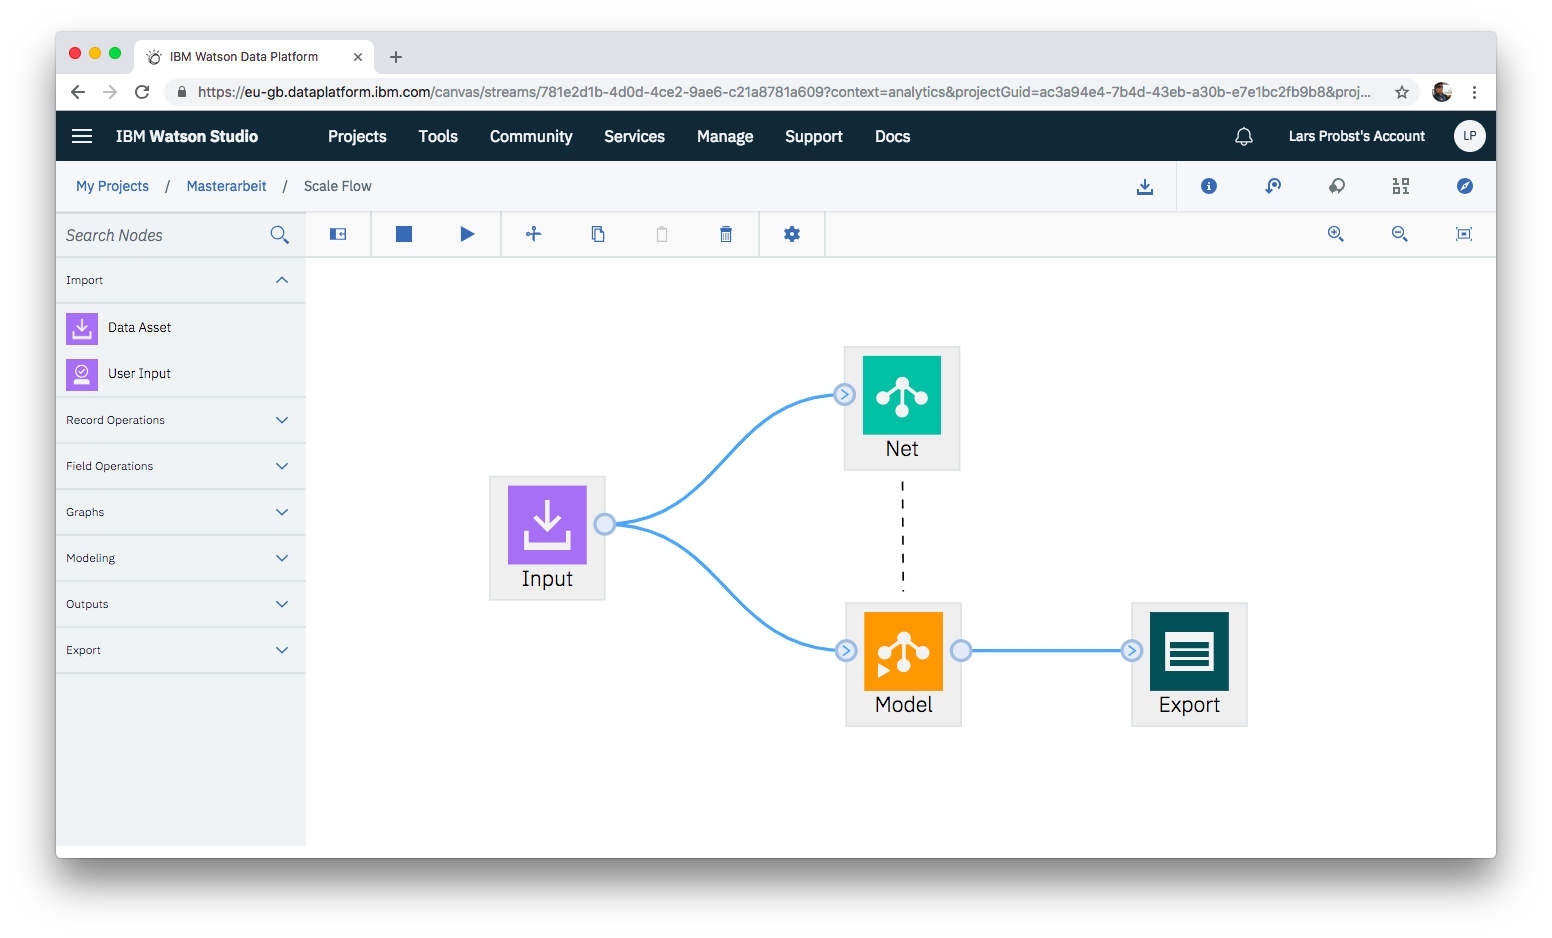
\includegraphics[scale=0.26]{images/kapitel_3/umsetzung_model_flow.png}
    \caption{Vollständiger Model flow}
    \label{fig:umsetzung_model_flow}
\end{figure}

\subsubsection{Informationen zum Model}
Über ein weiteren rechtsklick auf das trainierte Model und dem Menüpunkt \texttt{View Model} wird eine detaillierte
Übersicht über das Model angezeigt. In diesem finden sich zahlreiche Informationen die aufschluss über die Verwendbarkeit
des Models geben.

\colorbox{yellow}{Beschreiben von den ganzen Informationen von dem Model. Rechte Maustaste - View}

\begin{figure}[h]
    \centering
    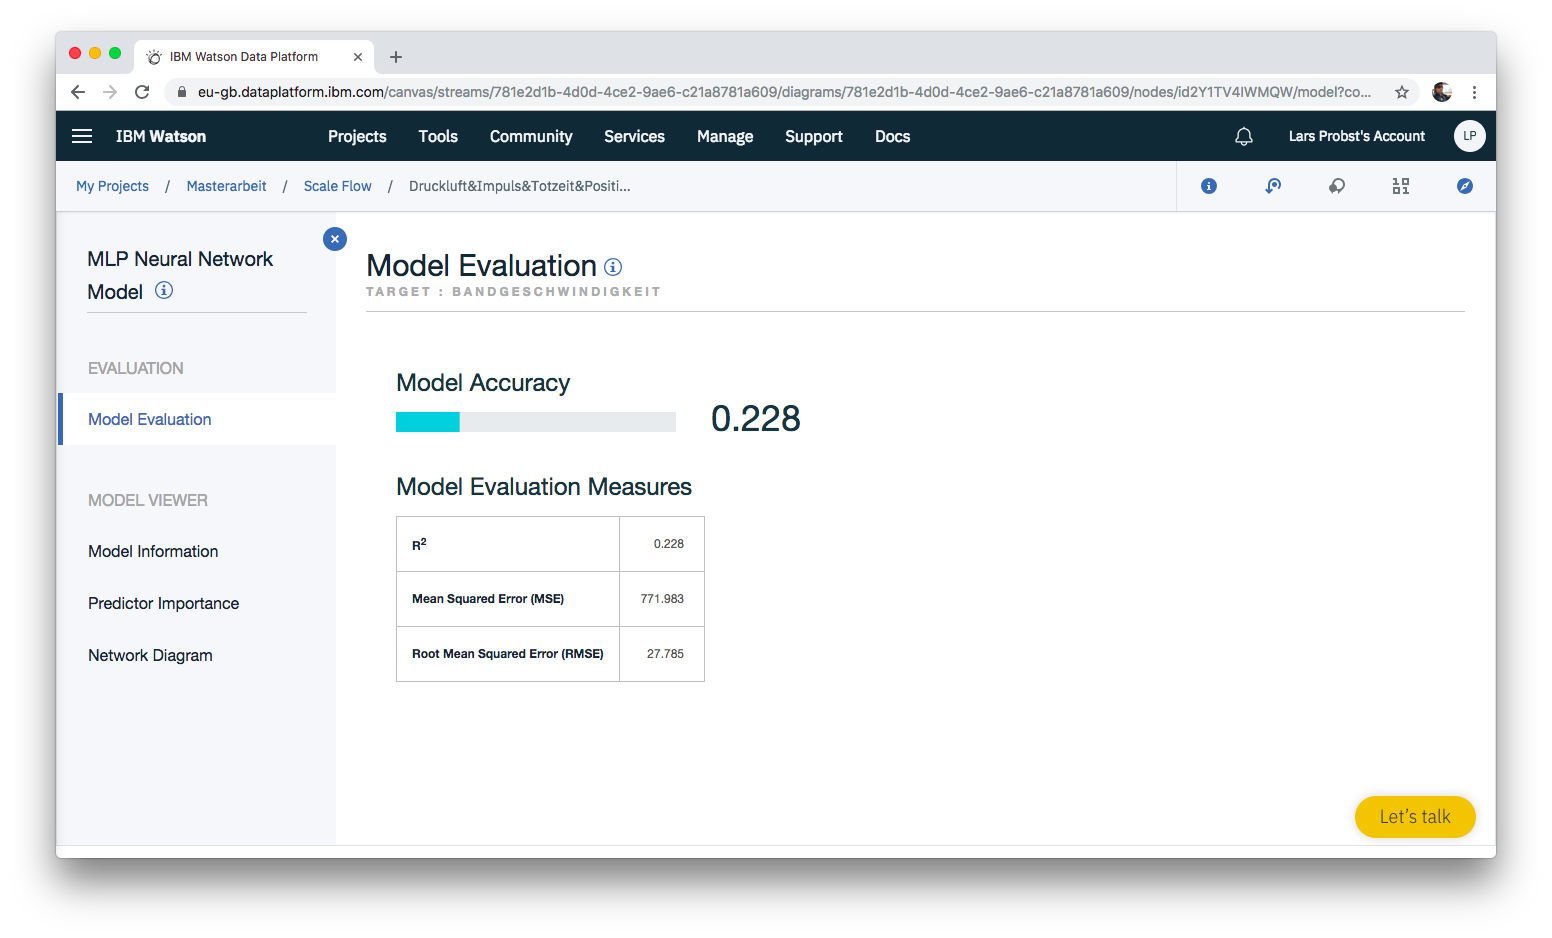
\includegraphics[scale=0.26]{images/kapitel_3/model_evaluation.png}
    \caption{Kompletter Model flow}
    \label{fig:umsetzung_model_evaluation}
\end{figure}

\begin{figure}[h]
    \centering
    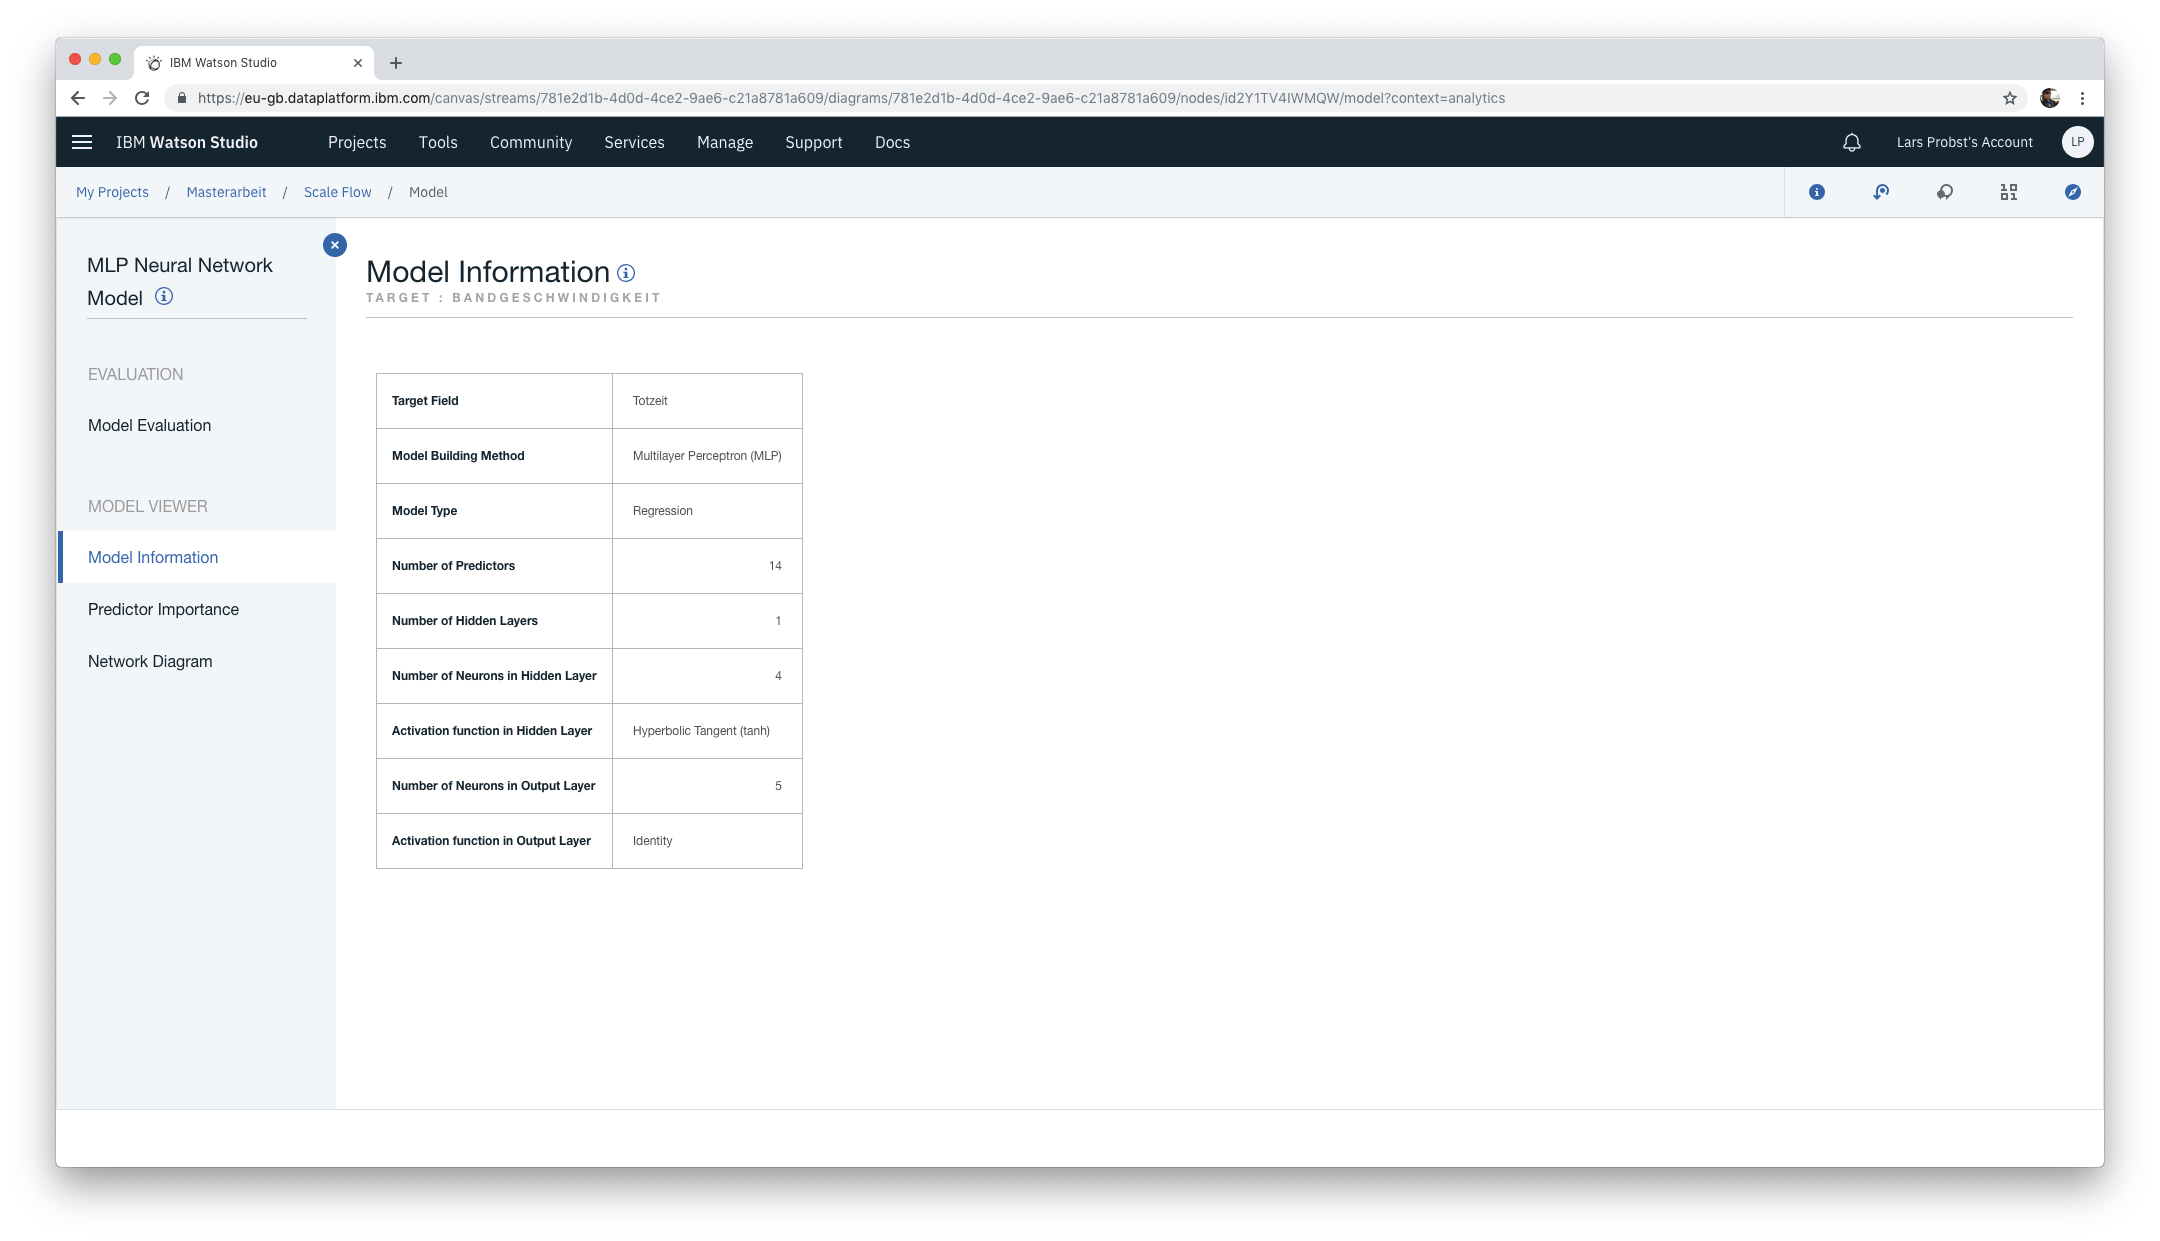
\includegraphics[scale=0.26]{images/kapitel_3/model_information.png}
    \caption{Kompletter Model flow}
    \label{fig:umsetzung_model_information}
\end{figure}

\begin{figure}[h]
    \centering
    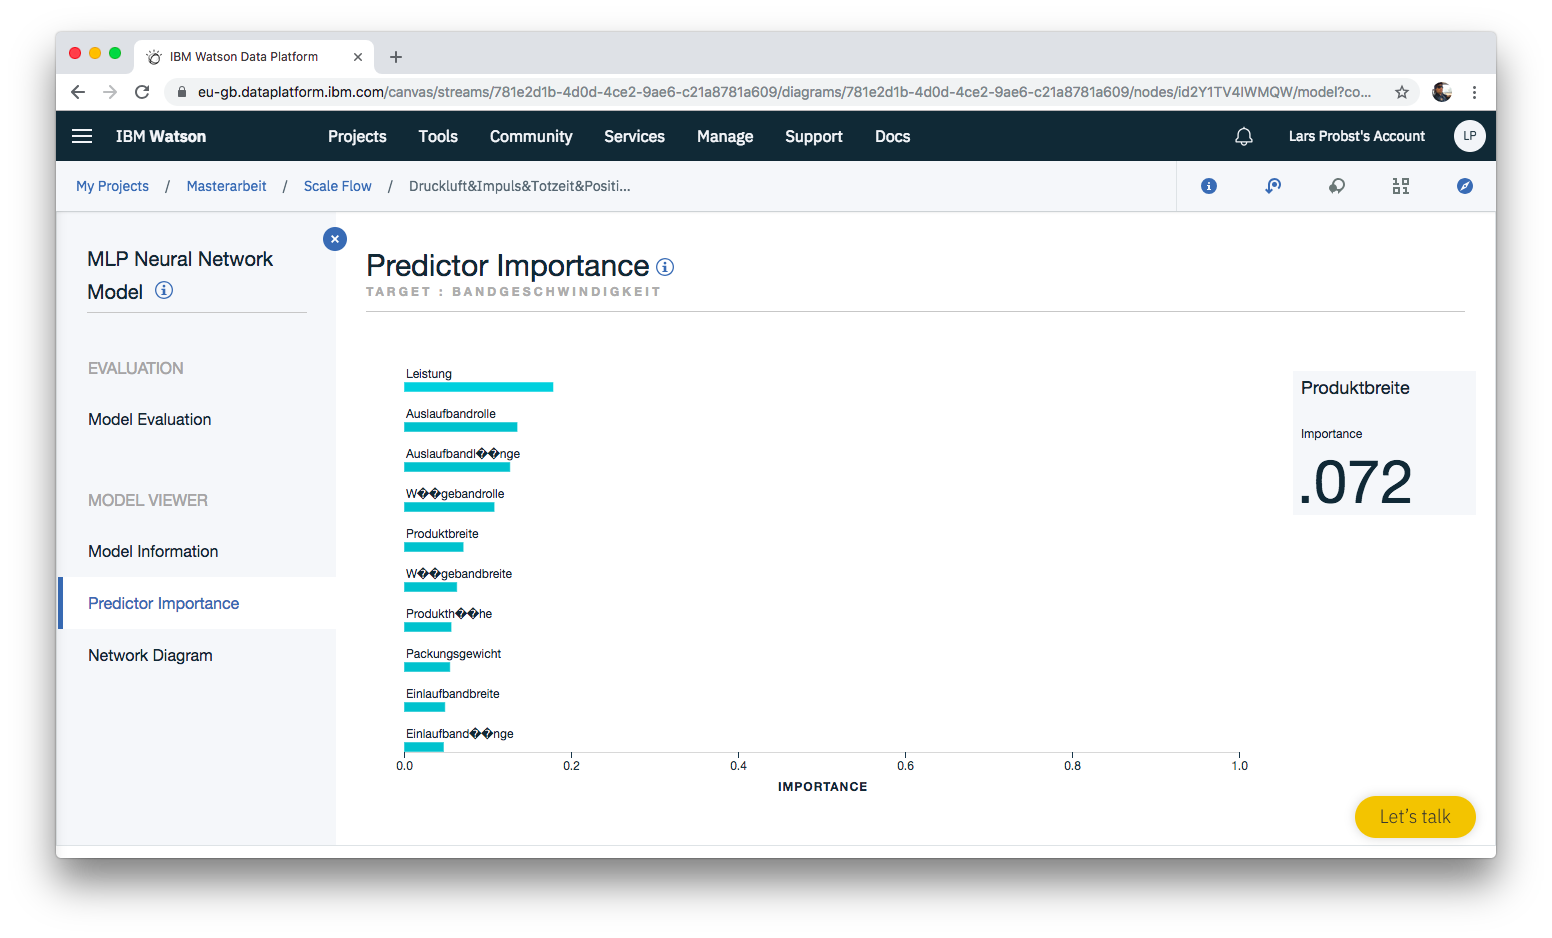
\includegraphics[scale=0.26]{images/kapitel_3/model_predictor.png}
    \caption{Kompletter Model flow}
    \label{fig:umsetzung_model_predictor}
\end{figure}

\begin{figure}[h]
    \centering
    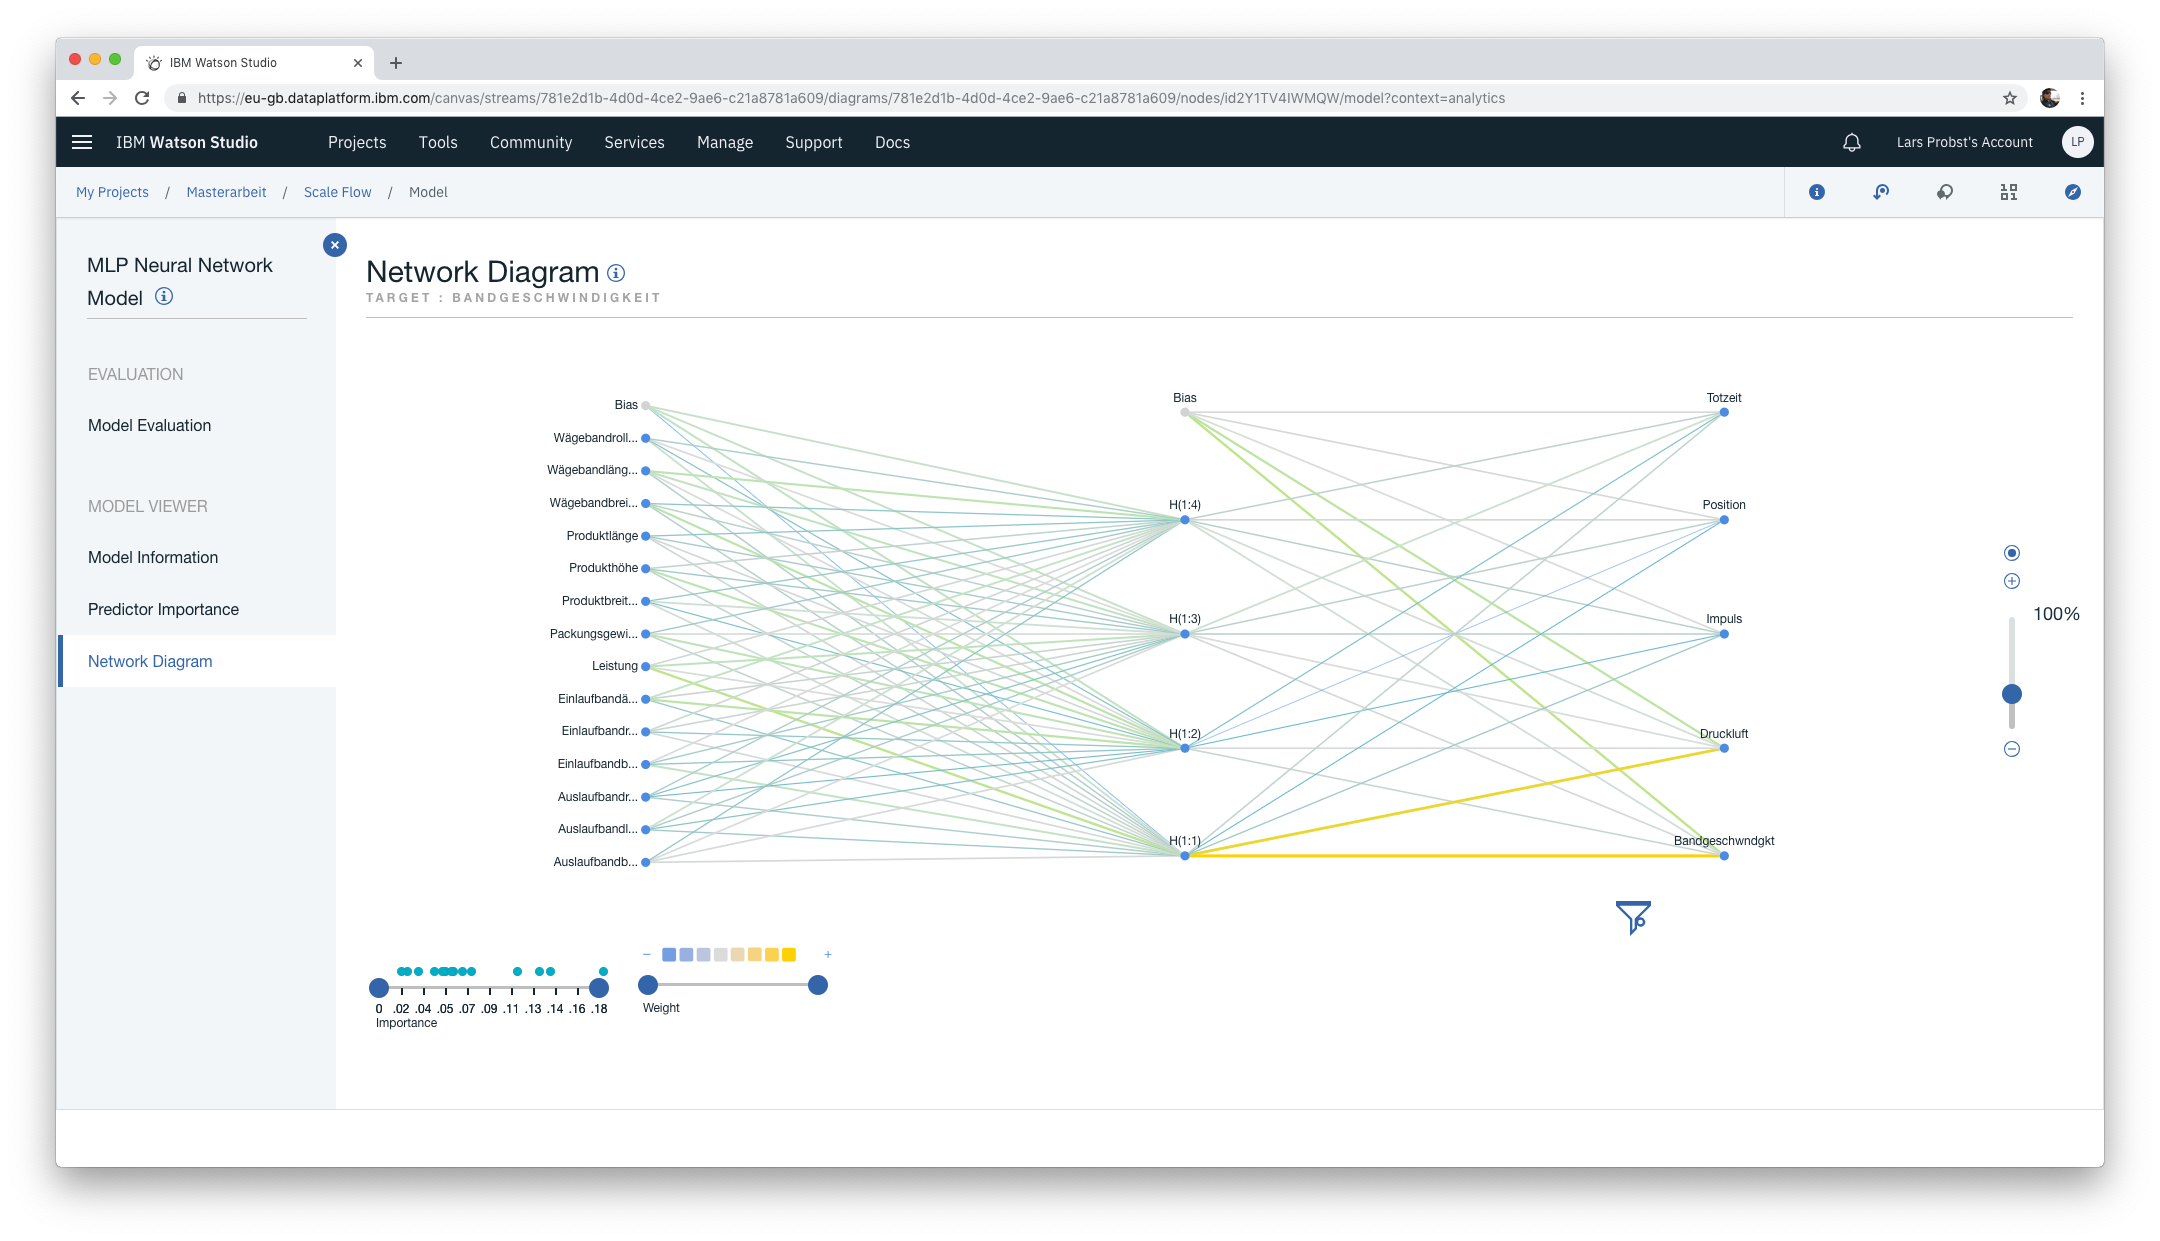
\includegraphics[scale=0.26]{images/kapitel_3/model_network_diagram.png}
    \caption{Kompletter Model flow}
    \label{fig:umsetzung_model_network_diagram}
\end{figure}

\subsubsection{Deployment erstellen}
Das im vorangegangenen Kapitel erstellte und trainierte Model kann im weiteren durch ein Deployment über eine
REST-Schnittstelle verfügbar gemacht werden. Dazu ist es erforderlich, das Model in einen \texttt{Web service} zu
installieren. Die spätere Wartung und Verwaltung wird dabei von Bluemix übernommen.

Für die Erstellung des Web Services wird im Watson Dashboard das erstellte Model ausgewählt. Das folgende Fenster
zeigt mehrere Informationen zu diesem an. Unter anderem ist sichtbar, welche Eingabe- und Ausgabeparameter für das Model
wichtig sind.

Der Reiter  \texttt{Evaluation} zeigt vorangegangene Auswertungen des Models an. Über den Menüpunkt \texttt{Lineage}
werden Verknüpfungen und Abstammungen des Models angezeigt.

Für das Deployment ist der Reiter \texttt{Deployments} wichtig. Dieser verwaltet alle Deployments des Modules. Das Löschen
von älteren Deployments oder das Erstellen von neuen ist hier möglich. Die Schaltfläche \texttt{Add Deployment} öffnet
eine Konfigurationsseite zum Erstellen eines neuen Deployments.

Der \texttt{Type} des Deployments ist Web Service. Der Name des Deployments ist das einzige Pflichtfeld und muss befüllt
sein. Anschließend wird das Deployment über \texttt{Save} gespeichert und gestartet. Dieser Vorgang kann wenige Minuten
dauern.

Nachdem das Deployment fertiggestellt ist, wird in der Spalte \textit{Status} der aktuelle Wert \texttt{DEPLOY\_SUCCESS}
angezeigt. Die Informationsseite des Deployments öffnet sich über einen klick auf den Namen.

Das Deployment ist somit erfolgreich erstellt und kann im weiteren getestet und genutzt werden.

\subsubsection{Deployment testen}
Ein online Test des eingerichteten Deployments ist über das Watson Studio Dashboard möglich. Dies hat den Vorteil, dass
das Deployment direkt getestet und bei Fehlveralten neu trainiert werden kann.

Auf der Deploymentseite des gespeicherten Models genügt ein klick auf den Namen um die Deploymentinformationen anzuzeigen.
Hier steht neben diversen Informationen auch der Menüpunkt \texttt{Test} zur Verfügung. In diesem öffnet sich eine
zweispaltige Ansicht. In der linken Spalte befinden sich die Eingabefelder für das trainierte Model. Nach der Eingabe
der Werte startet die Vorhersage über die Schaltfläche \texttt{Predict}.

Nach wenigen Sekunden erscheint auf der rechten Seite ein langes JSON-Object, welches den Rückgabewert des Web Services
aufzeigt. Das erste Array, \textit{fields}, listet alle an den Web-Service gesendeten Felder auf.

Das zweite Array, \textit{values}, die an den Web-Service gesendeten wie auch die Vorhergesgaten Werte.
Die letzten fünf Werte des Arrays entsprechen den Vorhersagen des trainierten Models.

Sollte das Array \textit{values} kleiner sein als das Array \textit{fields}, war das trainieren des Models nicht
erfolgreich.

Unter dem Menüpunkt \texttt{Implementation} werden wichtige Informationen und erforderliche Schritte aufgezeigt, damit
die Schnittstelle in das eigene Programm integriert werden kann. Dabei wird auf verschiedene Programmiersprachen
eingegangen.

\begin{figure}[h]
    \centering
    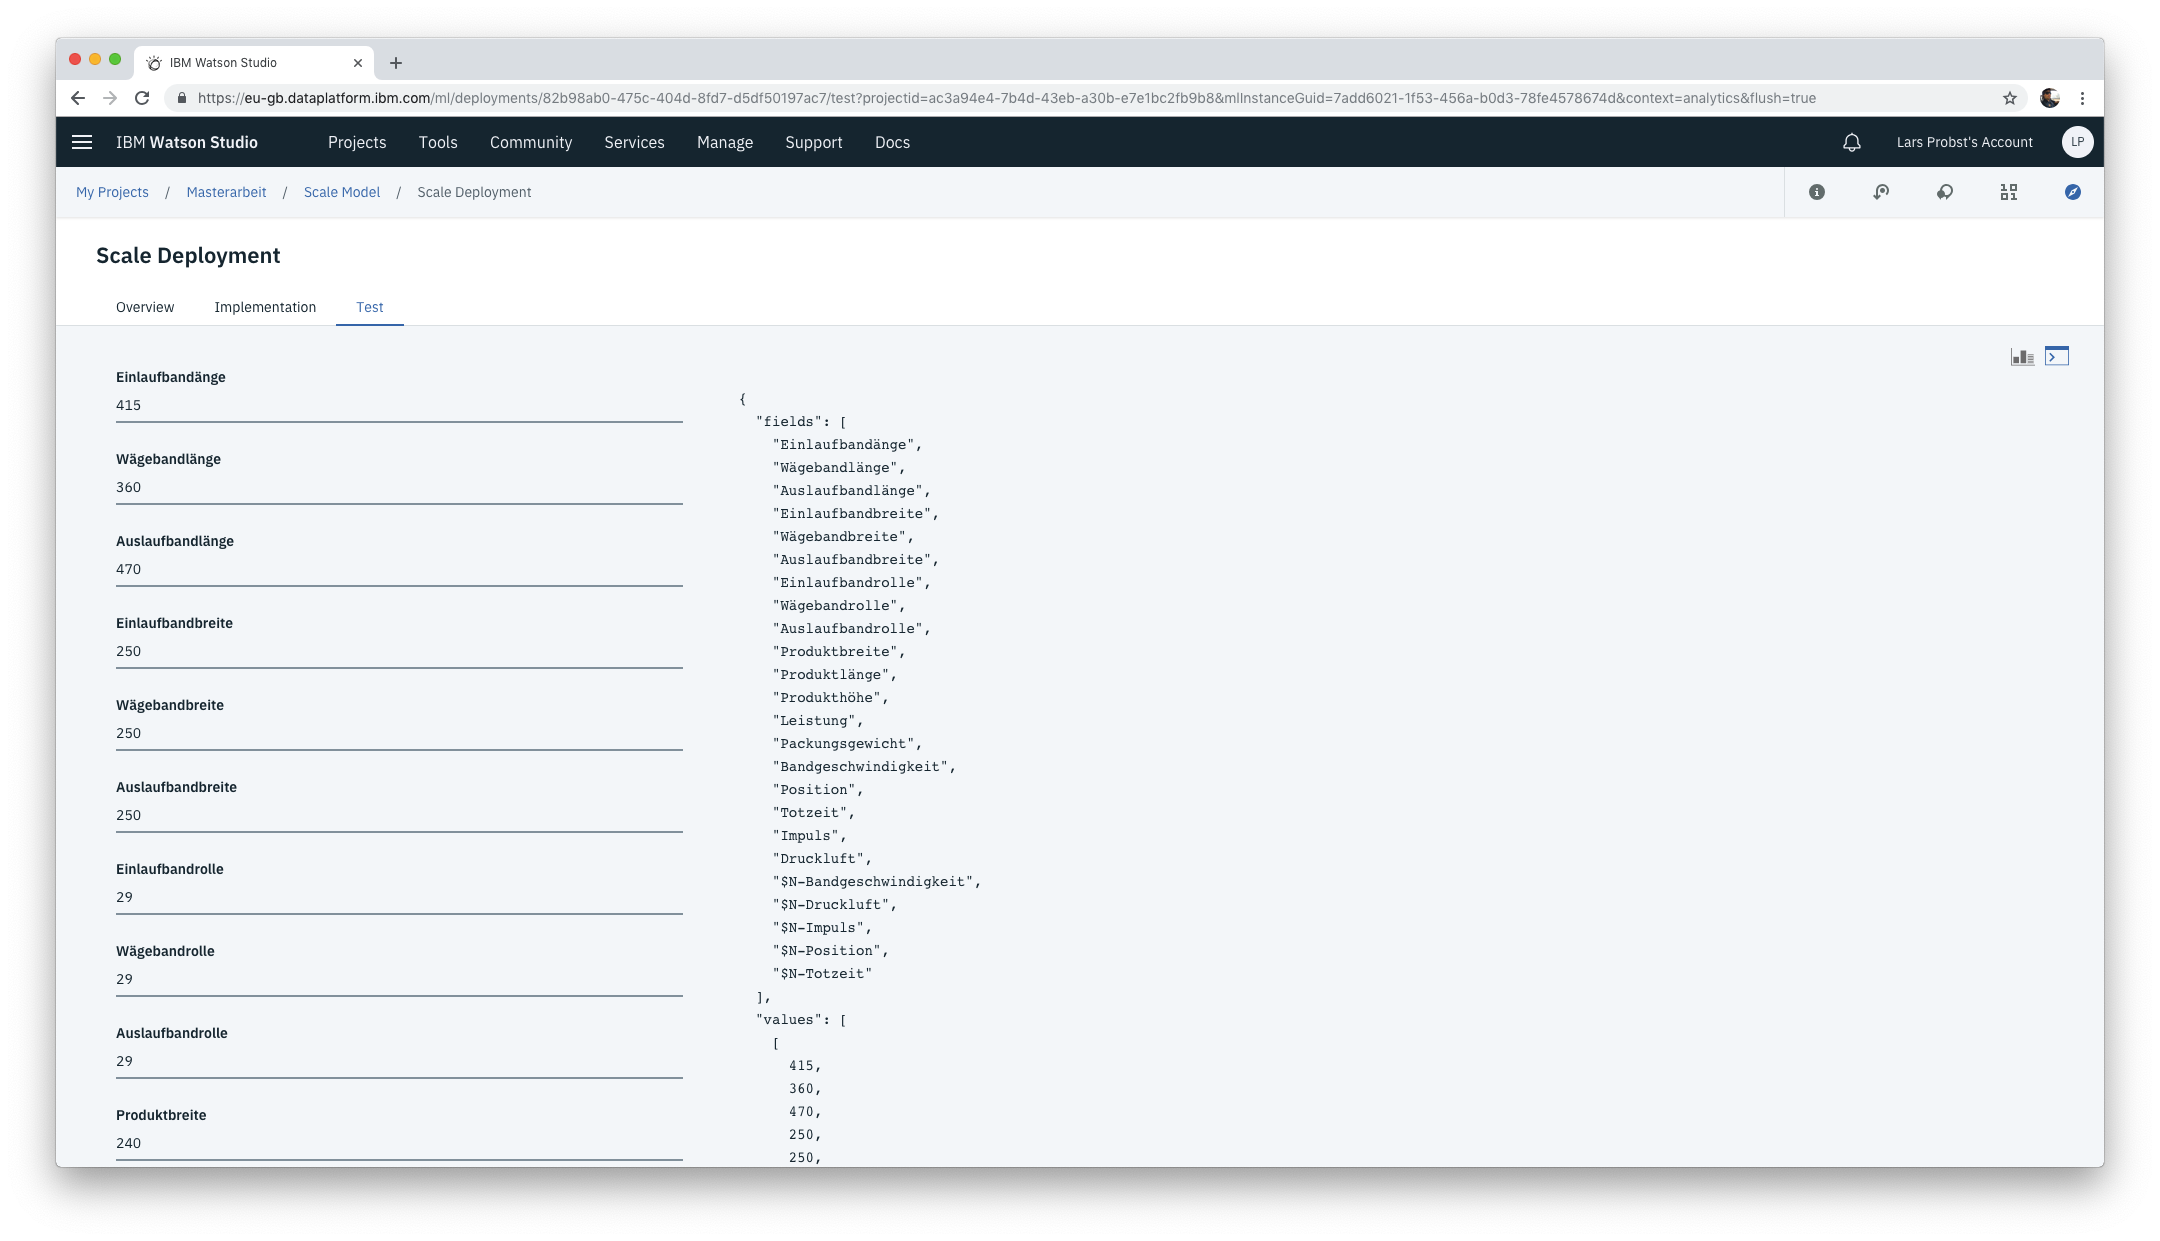
\includegraphics[scale=0.26]{images/kapitel_3/deployment_test.png}
    \caption{Kompletter Model flow}
    \label{fig:umsetzung_deployment_test}
\end{figure}

\subsubsection{Aufruf mit Postman}
\label{subsec:Aufruf mit Postman}
Im Weiteren soll das erstellte Model, welches über ein Deployment in einem Web-Service zur Verfügung gestellt wurde,
mit Postman\footnote{https://www.getpostman.com} getestet werden.

So ist sichergestellt, dass das Model auch von extern, nicht nur über das Watson Studio Dashboard, aufrufbar ist.
Dies ist für die spätere Entwicklung des Frontends und die Einrichtung des API Connect Services wichtig. Außerdem ist
so eine überprüfung der Übergabeparameter sowie der Rückgabewerte an die Schnittstelle möglich.

Jeder Request an den Web-Service des trainierte Models benötigt einen \textit{Authentication Token} (kurz Auth-Token).
Dieser Token stellt sicher, dass es sich um einen gültigen Aufruf handelt.

Über die REST-Schnittstelle des Watson Studios wird der Token generriert. Dabei handelt es sich um eine andere
Schnittstelle als beim Web-Service. Der Token ist immer nur für maximal vier Stunden gültig.

Um einen Auth-Token zu erstellen, muss der Watson Studio Benutzername und das zugehörige Passwort an die Schnittstelle
übergeben werden. Ein Beispielaufruf ist in Listing~\ref{Abruf des Auth-Tokens} auf Seite~\pageref{Abruf des Auth-Tokens}
zu sehen. Der Token ist dabei in einem JSON-Object im Rückgabewert enthalten.

\begin{lstlisting}[language=bash, caption=Abruf des Auth-Tokens, label=Abruf des Auth-Tokens]
$ curl --basic --user USERNAME:PASSWORD https://eu-gb.ml.cloud.ibm.com/v3/identity/token
\end{lstlisting}

In Postman ist dieser Aufruf durch die Eingabe der URL und dem HTTP-Type \texttt{GET} möglich. Im Reiter
\textit{Authentication} ist der Type \textit{Basic-Auth} auszuwählen.

Im rechten Bereich sollten dann die beiden Eingabefelder für Benutzername und Passwort erscheinen. Nach der Eingabe der
geforderten Daten wird der Request mit \texttt{Send} abgeschickt. Nach wenigen Sekunden erscheint im Bereich
\textit{Body} der Token in einem JSON-Objekt. Ähnlich dem Aufruf mit \textit{curl}.

Um nun das eigentliche Deployment aufzurufen, wird ein neuer Postman-Tab geöffnet. Die URL für den Endpunkt ist im
Deployment des Models zu finden und heißt \texttt{Scoring End-point}.

Nun kann der Scoring End-point als URL in Postman eingetragen werden. Als HTTP-Type ist \texttt{POST} auszuwählen.
Im Bereich \texttt{Authentication} wird der Typ auf \texttt{Baerer} abgeändert und ermöglicht die Eingabe des Tokens.

Die Auswahl des HTTP-Types \textit{POST} ermöglicht die definition des Bereichs \texttt{Body} für den Request. Dabei
handelt es sich um Parameter, welche an die Schnittstelle mitgeschickt werden. Als Datentyp wird \textit{raw} und als
Type \textit{JSON (application/json)} ausgewählt. Im Anhang \ref{sec:postmanTestparameter} auf Seite
\pageref{sec:postmanTestparameter} sind Testparameter zu finden, welche als Eingabe genutzt werden können.

Abschließend wird über den Button \texttt{Send} der Request an den Web Service abgeschickt. Nach wneigen Sekunden zeigt
Postman den erhaltenen Response des neuronalen Netzes an. Hier sollten auch die Vorhersagen enthalten sein.

Auf der Übersichtsseite des REST-Interfaces des
Deployments\footnote{https://watson\-ml\-api.mybluemix.net/?cm\_mc\_uid=61889453441915363064337}, sind noch weitere
Endpunkte und die dafür benötigten Parameter sowie die Rückgabewerte ersichtlich.

\begin{figure}[h]
    \centering
    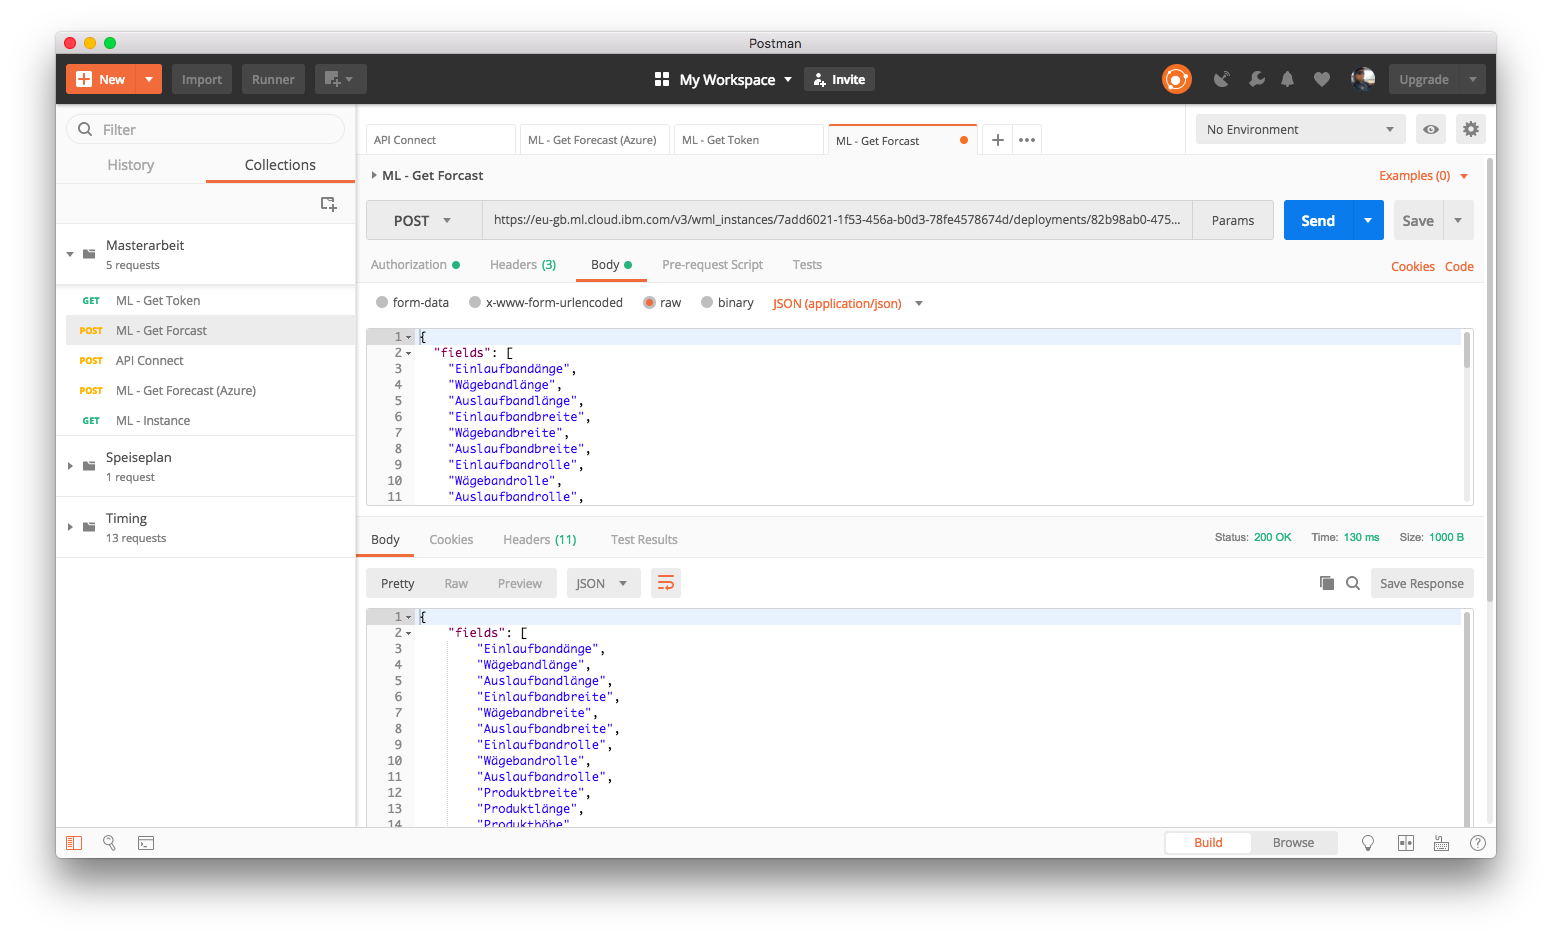
\includegraphics[scale=0.26]{images/kapitel_3/deployment_postman.png}
    \caption{Beispielrequest von Postman}
    \label{fig:umsetzung_deployment_postman}
\end{figure}

\subsection{TensorFlow.js}
Die Watson Studio Applikation ist nun erfolgreich in einem Deployment, online zur Verfügung gestellt. Außerdem ist die
Funktion über einen Aufruf mittels Postman überprüft worden. Im Weiteren wird das trainierte Model in eine TensorFlow.js
Applikation eingebaut.

\colorbox{yellow}{Hier fehlt was}

\subsubsection{Model Exportieren}
\colorbox{yellow}{Hier fehlt was}

Die Applikation soll im Weiteren über eine Domain aus dem Internet aufrufbar sein. Eine Installation in einen Cloud
Foundry-Container, welcher in der IBM Cloud läuft, ist dafür notwendig. Im folgenden Kapitel werden die dafür nötigen
Schritte erläutert.

\subsection{Toolchain einrichten}
Die fertig entwickelte Node.js-Applikation wird im nächsten Schritt in einen Cloud Foundry-Container installiert. Dies
ermöglicht den Aufruf der Applikation über eine Domain. Damit der geschriebene Quellcode nicht nach jeder änderung manuell
mittels \texttt{cf push} in einen Cloud foundry-Container geladen werden muss, wird hierfür eine Toolchain aus der
IBM Cloud genutzt.

Die Nutzung der Toolchain erfordert ein eingerichtetes Git-Repository. Nach jedem \texttt{commit}, welcher in dieses
Repository geschrieben wird, aktiviert sich die Toolchain selbstständig und lädt den entsprechenden Commit herunter.

Anschließend werden, je nach gewählter und eingerichteter Konfiguration, verschiedene Schritte (Phasen) in der Toolchain
durchlaufen, um die Applikation in einen Cloud Foundry-Container zu installieren.

Dabei können die einzelnen Schritte, welche beim Deployment durchlaufen werden, selbst definiert, oder eine
vorkonfigurierte Toolchain genutzt werden. Die vorkonfigurierte Toolchain kann im Nachgang allerdings individuell
angepasst werden und dient lediglich einem schnelleren Start.

Für die Konfiguration der Toolchain muss die instanziierte Node.js-Runtime, in welcher die entwickelte Applikation laufen
soll, in dem IBM Cloud Dashboard ausgewählt werden.

Auf der folgenden Seite, im Tab \texttt{Übersicht} (linke Seite), erscheinen fünf Kacheln mit unterschiedlichen Informationen.
Für die Toolchain ist die Karte mit der Aufschrift \texttt{Continous Delivery} entscheidend. Dort gibt es einen Button
mit der Aufschrift \texttt{Aktivieren}.

Ein Klick auf diesen öffnet die Übersicht und eine visuelle Vorschau der Standardkonfiguration der Toolchain. Nun kann
ein Name eingetragen und die Region ausgewählt werden, in der die Toolchain installiert werden soll. Da die
Standardkonfiguration vorerst völlig ausreichend ist, kann diese direkt übernommen werden. Dafür genügt ein Klick auf
\texttt{Erstellen}.

Nach einem kurzen Ladevorgang ist die Toolchain eingerichtet und vorkonfiguriert. Es erscheinen nun vier Karten für
unterschiedliche Bereiche, in denen die IBM Cloud dem Entwicklungszyklus helfen kann.

Im Bereich \texttt{Nachdenken} wird ein Issue-Tracker konfiguriert, in dem zum Beispiel Bugs (Softwarefehler), welche
in der Software entdeckt werden, eingetragen, verwaltet und diskutiert werden können.

In \texttt{Codieren} stehen gleich zwei Kacheln zur Verfügung. Einerseits das konfigurierte Git-Repository, bei dem es
sich um ein auf IBM-Servern gehostetet GitLab handelt. Andererseits findet sich dort eine Web-IDE, auf Basis von Eclipse
Orion, mit der der Quellcode der Anwendung online editiert werden kann.

Im der letzten Kategorie, \texttt{Bereitstellen}, findet sich die Pipeline, welche im nächsten Schritt näher Erläutert
und eingerichtet wird. Ein Klick auf die Kachel mit der Aufschrift \texttt{Delivery Pipeline} öffnet diese.

Nach dem Laden der Seite erscheinen zwei sogenannte \texttt{Phasen} (engl. Stages). Jeder Schritt in der Delivery Pipeline
wird durch eine Phase symbolisiert. In einer Phase können zum Beispiel der Quellcode aus dem Git-Repository geladen, oder
die geschriebenen Tests durchgeführt werden.

Die Standardkonfiguration sieht in der \texttt{Build Stage} das Herunterladen des Quellcodes aus dem Git-Repository vor
und in der \texttt{Deploy Stage} das Einrichten eines Cloud Foundy-Containers.

Für die Node.js-Applikation reicht diese Konfiguration völlig aus, da keine zusätzlichen Installationen oder Einrichtungen
notwendig sind.

Als nächstes muss der geschriebene Quellcode der Applikation lediglich noch in das, in der Toolchain hinzugefügte,
Git-Repository eingecheckt werden. Die URL für das Repository kann in der Toolchain-Übersicht mit einem Klick auf die
Kachel \texttt{Git} angezeigt werden.

Nach erfolgreichem \texttt{push} der Anwendung in das Git-Repository startet der deployment Vorgang in der Toolchain
selbstständig. Nach wenigen Minuten sollte die Anwendung über ihre URL, welche in der Node.js Runtime definiert ist,
aufrufbar sein.

Da die Applikation nun im Internet in einem Cloud Foundry-Container zur Verfügung steht, kann diese im nächsten Schritt
mit dem API Connect Service verbunden werden. Dieser Schritt ist nötig, damit die Schnittstelle der Applikation vom
Frontend, welches in Kapitel~\ref{subsec:webseite} auf Seite~\pageref{subsec:webseite} beschrieben wird, und über Postman
vereinfacht aufgerufen werden kann.

\begin{figure}[h]
    \centering
    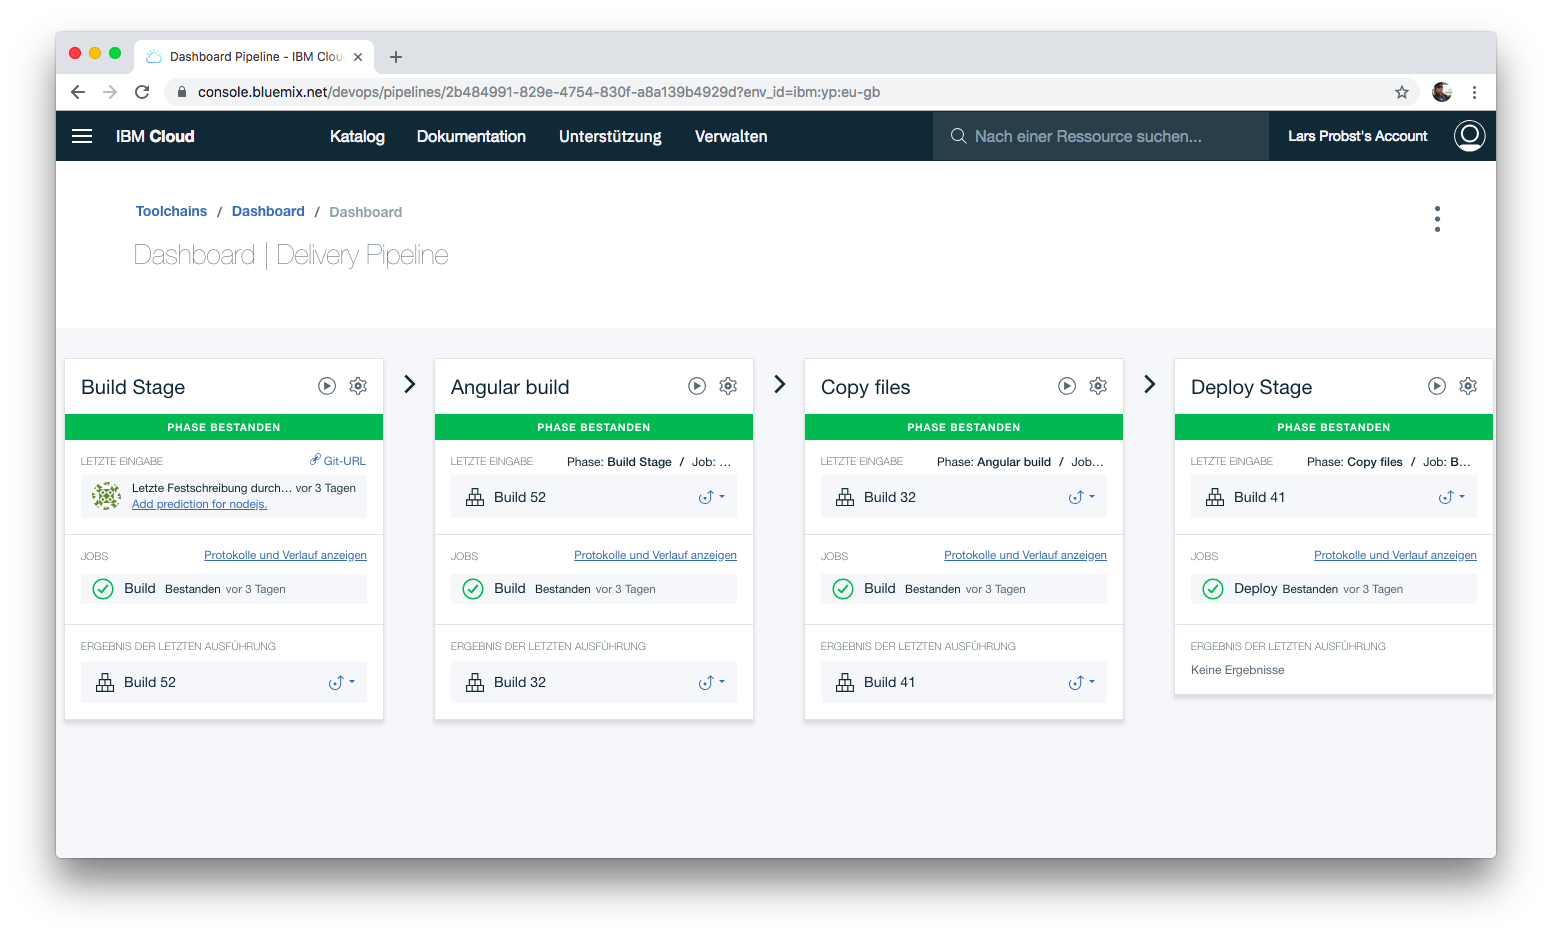
\includegraphics[scale=0.26]{images/kapitel_3/toolchain_pipeline.png}
    \caption{Übersicht der Toolchain-Konfiguration}
    \label{fig:umsetzung_toolchain_pipeline}
\end{figure}

\subsection{API Connect}
Wie in Kapitel \ref{subsec:Aufruf mit Postman} auf Seite \pageref{subsec:Aufruf mit Postman} beschrieben, benötigt das
REST-Interface des erstellten Deployments einen Auth-Token. Dieser kann nur über den Aufruf einer anderen
REST-Schnittstelle zur Verfügung gestellt werden.

Damit dies vereinfacht werden und das im weiteren Verlauf erstellte Frontend ebenfalls das Deployment aufrufen kann,
werden beide Abfragen in API Connect gebündelt.

Ein weiterer Grund für das Bündeln der beiden Anfragen an den Watson Service ist das mitschicken des Benutzernamens und
des zugehörigen Passwortes zum generrieren des Tokens. Damit diese nicht in der zu entwickelnden Anwendung hinterlegt
werden müssen, können diese Zentral in API-Connect gespeichert werden.

Das hat den Vorteil, dass sie bei Bedarf nur an einer Stelle abgeändert werden müssen. Auch werden sie nicht in einer
Anwendung hinterlegt, in der sie relativ einfach abgefangen und zu anderen Zwecken genutzt werden können.

Ein weiterer Vorteil für die Nutzung von API Connect ist die Tatsache, dass es zwei Möglichkeiten gibt, Vorhersagen zu
beziehen. Nebem dem Deployment des Watson Models kann auch die Schnittstelle der Node.js-Applikation mit TensorFlow.js
genutzt werden.

Mittels API Connect können Aufrufe optimal verteilt und Änderungen können schnell und komfortabel mit einem Online-Editor
angepasst werden.

\subsubsection{API Connect einrichten}
Der in Kapitel \ref{subsec:apiconnect} auf Seite \pageref{subsec:apiconnect} eingerichtete Service wird im folgenden
konfiguriert und eingerichtet. Dazu muss er aus dem IBM Cloud Dashboard heraus aufgerufen werden.

\colorbox{yellow}{Hier fehlt was}

In der Abbildung \ref{fig:umsetzung_api_connect} auf Seite \pageref{fig:umsetzung_api_connect} ist der fertig
eingerichtete API Connect Flow dargestellt.

\begin{figure}[h]
    \centering
    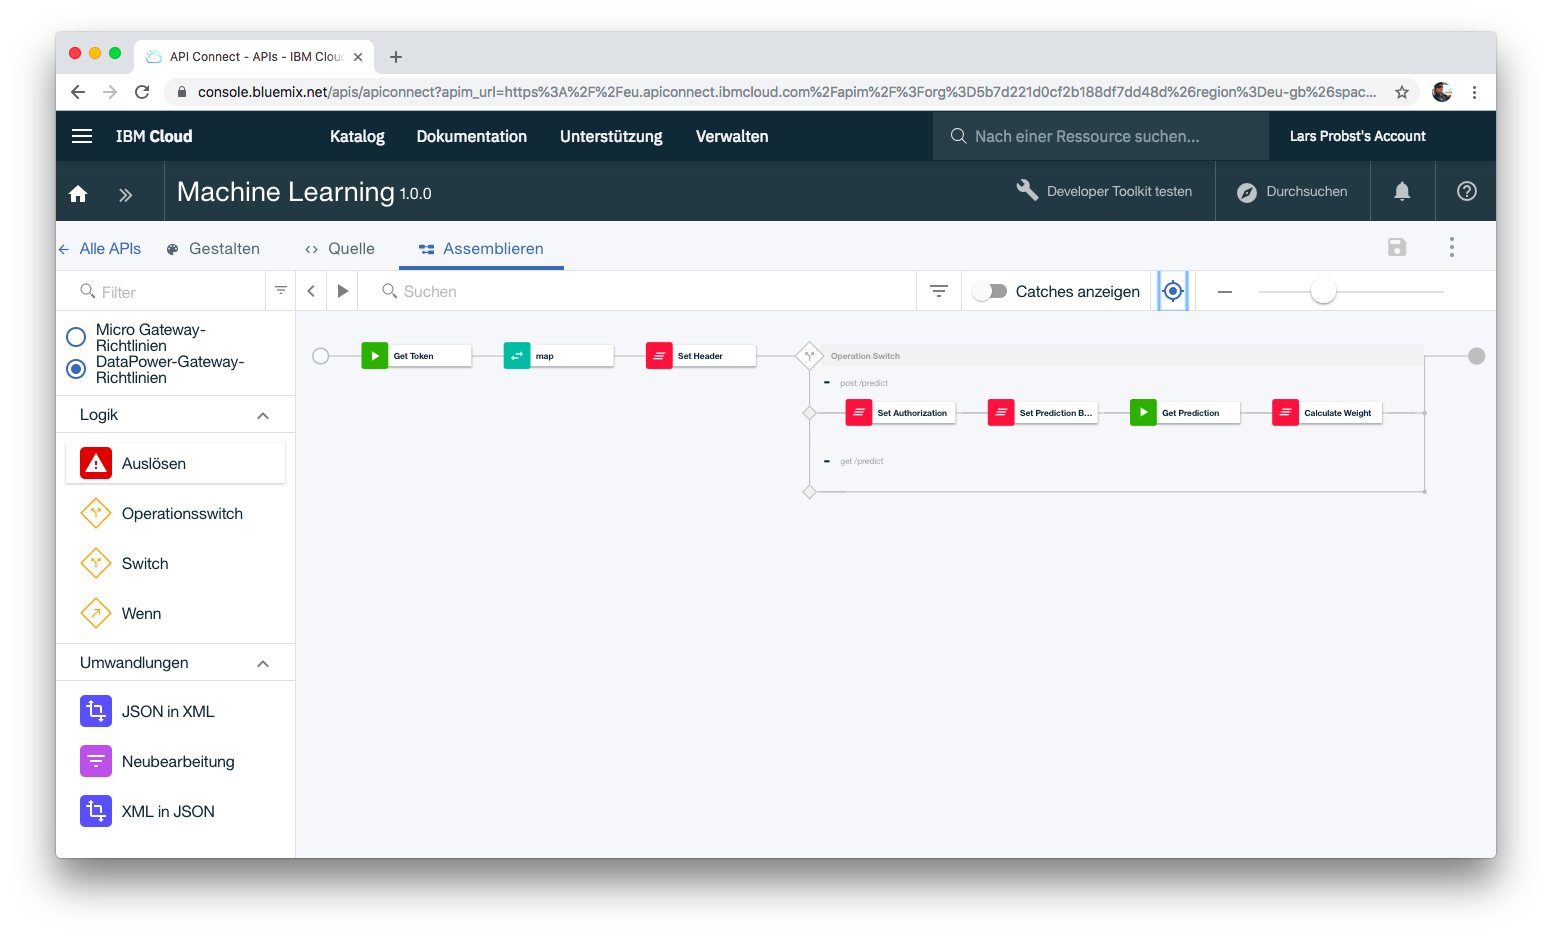
\includegraphics[scale=0.26]{images/kapitel_3/api_connect.png}
    \caption{Kompletter Model flow}
    \label{fig:umsetzung_api_connect}
\end{figure}